	\clearpage
\section{Firmware}\label{sec:Firmware}

\todo[inline]{Eine Hardwareplattform. Dongle mit Akku für die BSN und DK für den BMN. Firmware dementsprechend gibt es folgende: BMN, BSN Sensor, BSN Aktor}

\todo[inline]{Räffu: Mesh-5, 7, 8, 9}
\newpage


\subsection{Durchsatz Messung}\label{subsec:DurchsatzMessung}
\todo[inline]{Robin: Mesh-1, 3, 4}
Der Durchsatz wird gemessen, indem ein Client eine fixe vordefinierte Payload an den Server schickt. Die Zeit, die das Paket braucht um Vollständig übertragen zu werden, wird gemessen. Aus dieser Zeit und der Payload wird der Durchsatz berechnet. Für die Durchsatzmessung sind zwei verschiedene Modi vorgesehen. Der erste Modus misst den Durchsatz ohne applikations Acknowledgment vom Server und der zweite Modus mit Acknowledgement. Im Bild \ref{fig:KonzeptDurchsatzmessung} sind beide Varianten beschrieben. Die Anzahl Messungen kann vor dem Test definiert werden. 

\begin{figure}[H]
	\centering
	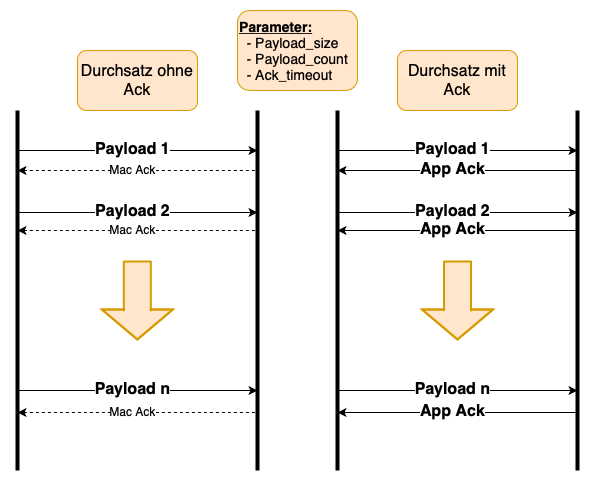
\includegraphics[width=0.5\textwidth]{Durchsatzmessung.png}
	\caption{Konzept Durchsatzmessung}\label{fig:KonzeptDurchsatzmessung}
\end{figure}

\subsection{Latenz Messung}\label{subsec:LatenzMessung}
Die Latenz beschreibt die Zeit, wie lange ein Paket hat bis es vollständig übertragen wurde. Da die Messung auf applikations Ebene stattfindet, wird die Zeit vom Funktionsaufruf des Clients bis zur Bestätigung vom Server gemessen. 

\begin{figure}[H]
	\centering
	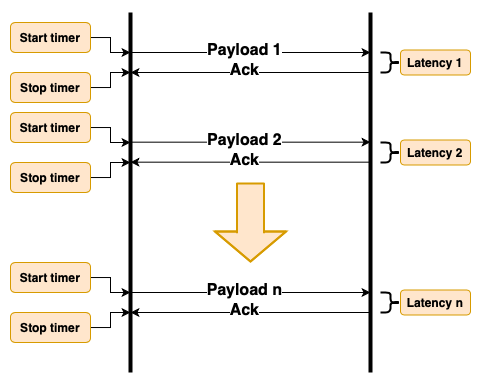
\includegraphics[width=0.5\textwidth]{Latenzmessung.png}
	\caption{Konzept Latenzmessung}\label{fig:Konzept Latenzmessung}
\end{figure}
\newpage



\todo[inline]{Cyrill: Mesh-2, 6, 10}


\subsection{Parameter Mesh Test}\label{subsec:ParameterMeshTest}



